\documentclass{beamer}

\usepackage[utf8x]{inputenc}
\usepackage[english]{babel}
\usepackage[export]{adjustbox}

\mode<presentation> {
	\usetheme{Berlin}
}

\usebackgroundtemplate {
	
\includegraphics[width=370px, height=270px, trim=0 0 0 -80px]{BackTriangles025.png}
}

\title[High Performance Conference, September 02-06, 2019, Borovets, Bulgaria]{
	Genetic Algorithm Based Formula Generation for Curve Fitting in Time Series Forecasting Implemented as Mobile Distributed Computing
}

\author{Rumen Ketipov, Georgi Kostadinov, Plamen Petrov,\\ Iliyan Zankinski, Todor Balabanov\textsuperscript{0000-0003-3139-069X}}

\date{02-06.IX.2019}

\institute[IICT-BAS, HPC'19] {
	Institute of Information and Communication Technologies \\ 
	Bulgarian Academy of Sciences \\
	\medskip
	\textit{todorb@iinf.bas.bg}
}

\addtobeamertemplate{navigation symbols}{}{
    \usebeamerfont{footline}
    \usebeamercolor[fg]{footline}
    \hspace{1em}
    \insertframenumber/\inserttotalframenumber
}

\begin{document}

\begin{frame}
\titlepage
\end{frame}

\begin{frame}
\frametitle{Agenda}
\tableofcontents
\end{frame}

\section{Introduction}

\begin{frame}
\center \huge{Introduction}
\end{frame}

\subsection{Time Series}

\begin{frame}
\frametitle{Financial Time Series}
\begin{itemize}
	\item Area of high researchers interest from many decades
	\item Having an accurate forecast in the financial world is crucial for many important decision makings
	\item Time series are ordered measurements of particular variable done in a temporal manner
	\begin{itemize}
		\item In the most cases values are measured on equal intervals
		\item But it is not a mandatory 
	\end{itemize}
\end{itemize}
\end{frame}

\begin{frame}
\frametitle{Time Series Forecasting}
\begin{itemize}
	\item It is applicable in processes with clear repetition pattern
	\item Measurements done in a temporal order are presented as points in a two-dimensional space
	\item Visually these points are connected with straight lines (simplified form of linear interpolation for the values between two neighboring measurements)
	\item In such two-dimensional space many different curves can be proposed for some generalization of the data nature (curve fitting problem)
	\begin{itemize}
		\item Linear regression can be used for trend estimation
		\item Lagrange polynomial as more complex generalization
	\end{itemize}
	\item {\color{red} Infinite number of curves can satisfy the condition to pass across finite number of points in two-dimensional space}
\end{itemize}
\end{frame}

\subsection{Evolutionary Computing}

\begin{frame}
\frametitle{Genetic Algorithms}
\begin{itemize}
	\item Meta-heuristic for global optimization inspired by the natural processes in the biological evolution
	\item Population based algorithms sub-class of the evolutionary algorithms
	\begin{itemize}
		\item Each individual is a vector into the solutions space
	\end{itemize}
	\item Based on three general operations - selection, crossover and mutation
\end{itemize}
\end{frame}

\begin{frame}
\frametitle{Optimization Remarks}
\begin{itemize}
	\item Proper encoding of the individuals (expression tree encoding in this study)
	\item Selection of parents (tournament selection in this study)
	\begin{itemize}
		\item With elitism rule applied
	\end{itemize}
	\item Crossover for exploration capabilities (single cut point in this study)
	\item Mutation for exploitation capabilities (random change of mathematical operation and random change of the operand in this study)
	\item Fitness value evaluation (curve fitting closeness in this study)
\end{itemize}
\end{frame}

\section{Experiments and Results}

\begin{frame}
\frametitle{Genetic Algorithm Parameters}
\begin{table}
	\begin{tabular}{p{5.4cm}p{4.4cm}}
		\hline
		\textbf{Parameter} & \textbf{Value} \\
		\hline
		generation gap & 0.97 \\
		crossover rate & 0.95 \\
		mutation rate & 0.03 \\
		maximum generations & 100 \\
		number of individuals & 37 \\
		number of variables & floating \\
		inserted rate & 100 \% \\
		\hline
	\end{tabular}
\end{table}
\end{frame}

\begin{frame}
\frametitle{EUR/USD Rate for Two Months}
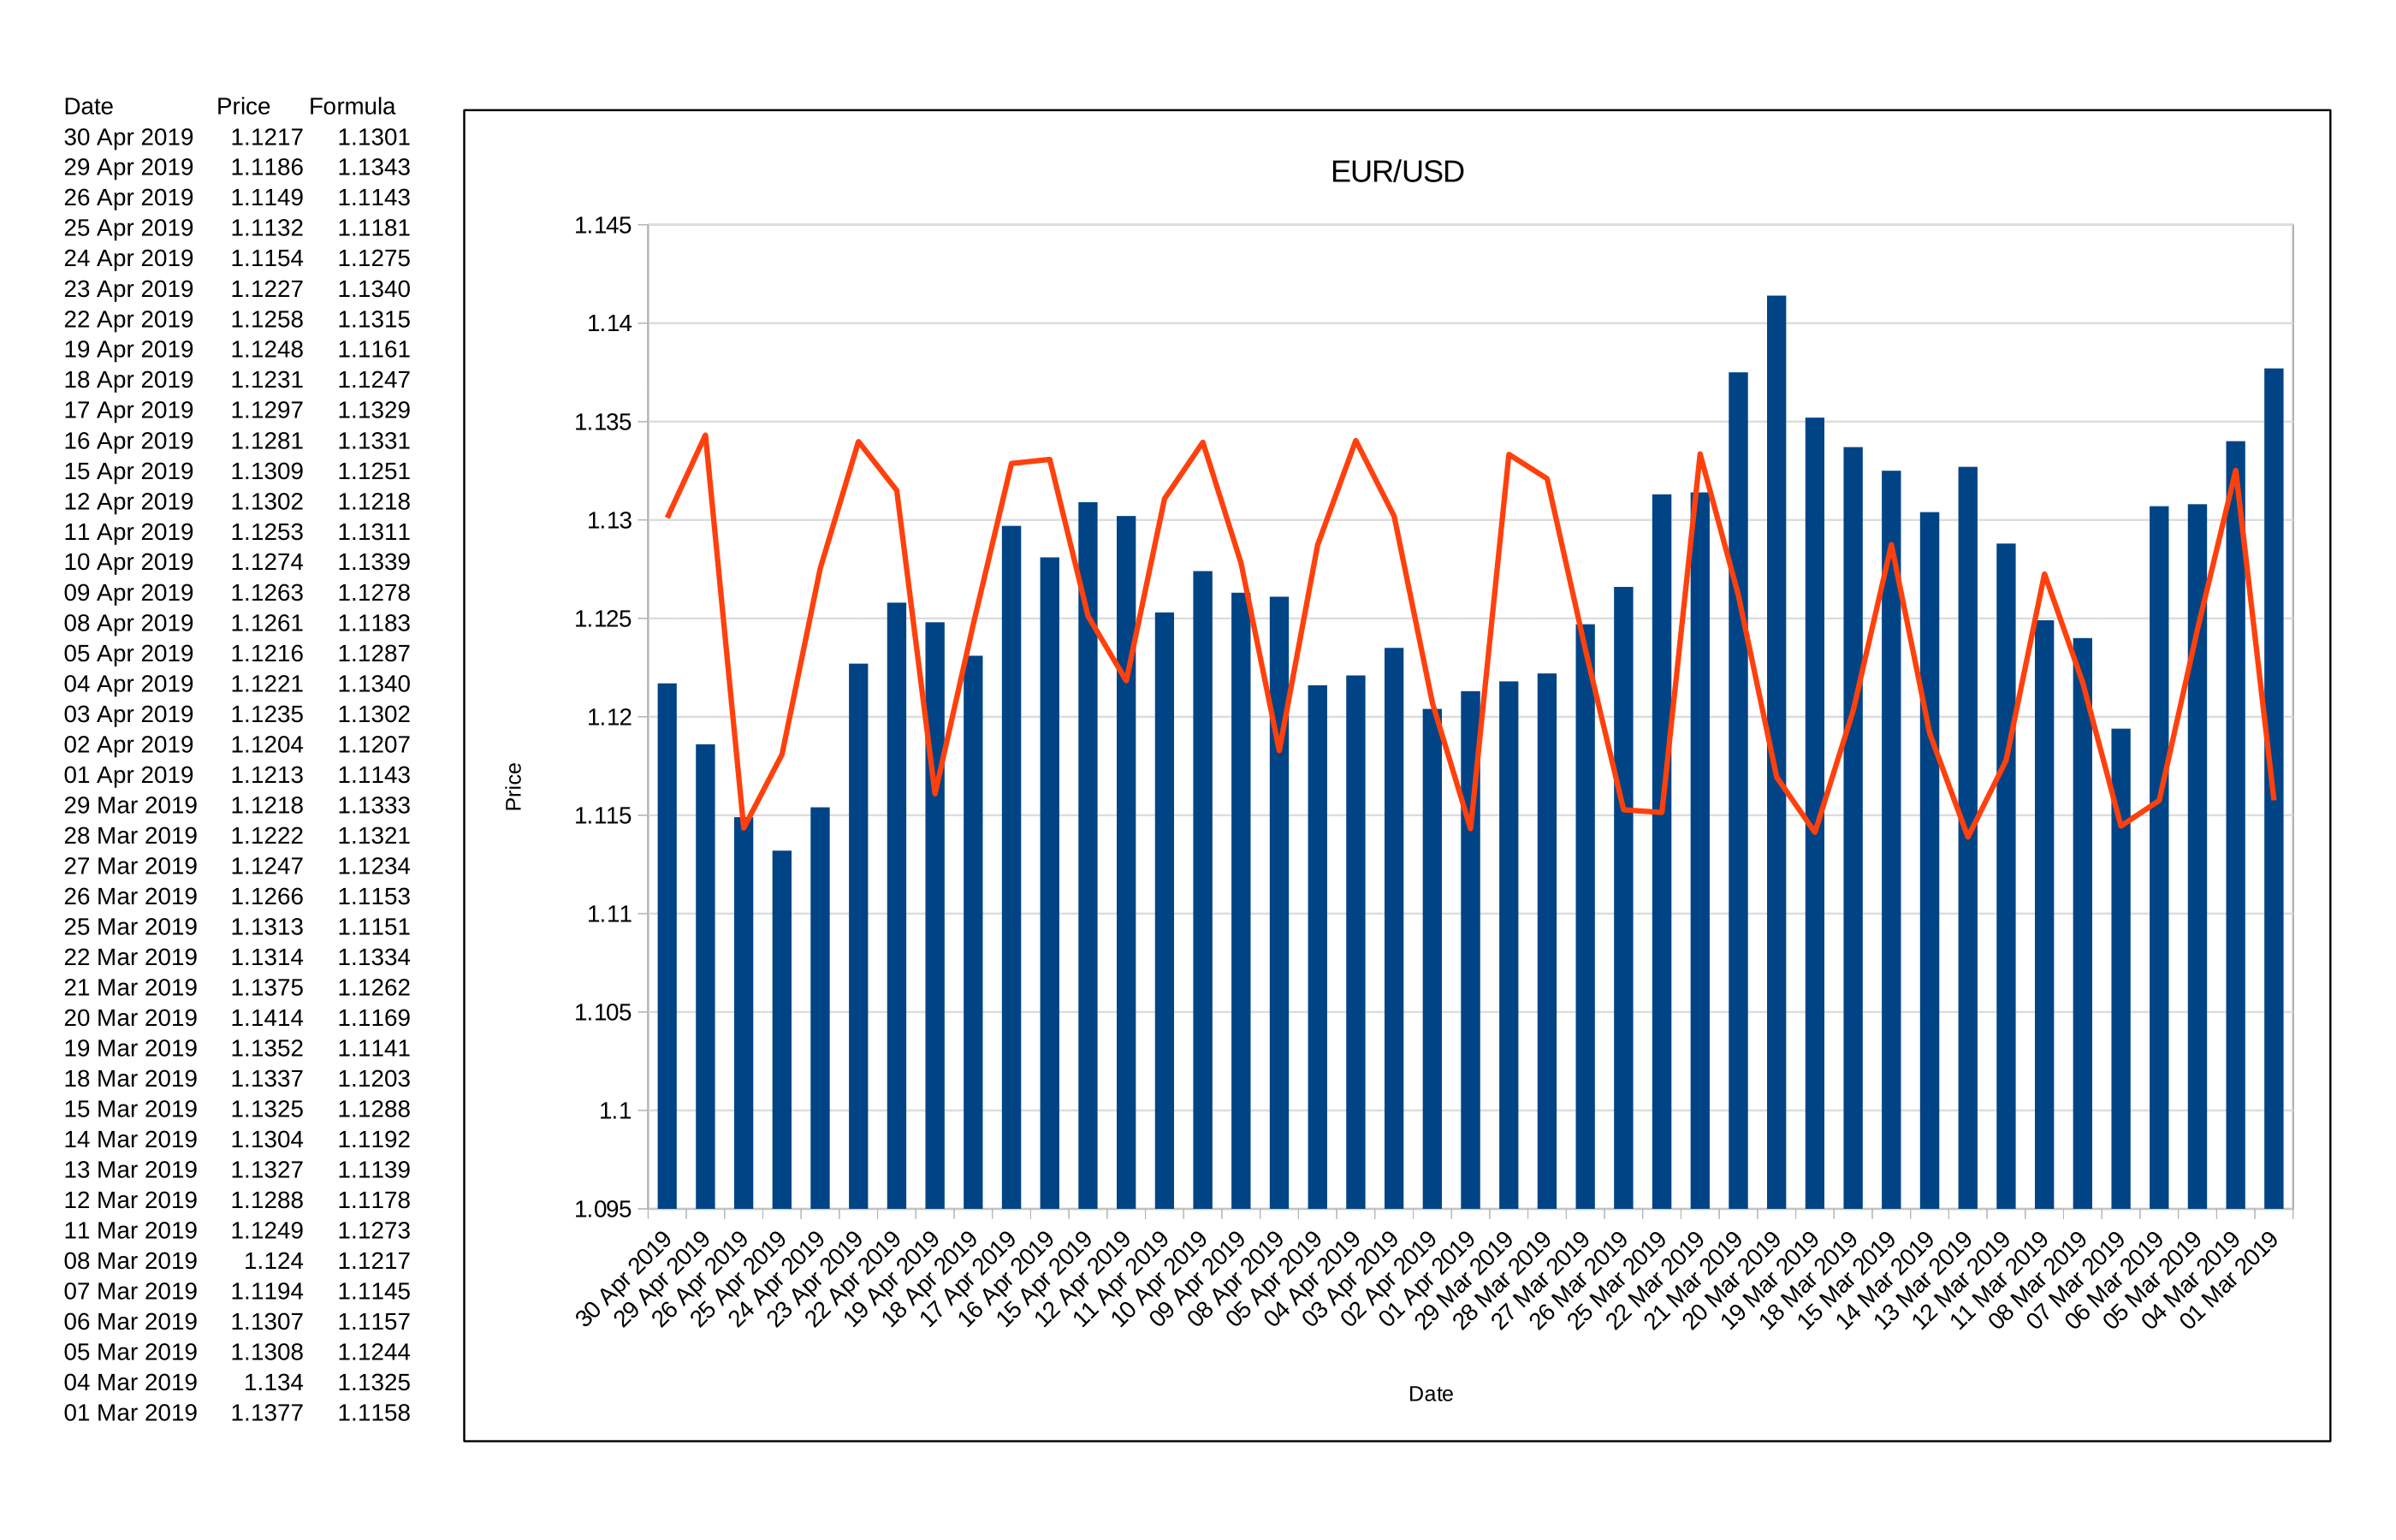
\includegraphics[scale=0.09]{fig01.png}
\end{frame}

\section{Conclusions}

\begin{frame}
\center \huge{Conclusions}
\end{frame}

\begin{frame}
\frametitle{Questions and Answers}
\center \huge{Thank you for the attention!}
\end{frame}

\end{document}